\documentclass[letterpaper]{article} % DO NOT CHANGE THIS
\usepackage{aaai2027}  % DO NOT CHANGE THIS (camera-ready style: MATH4AI review is single-blind)
\nocopyright  % non-archival workshop: the AAAI copyright line does not apply to this paper
\usepackage[hyphens]{url}  % DO NOT CHANGE THIS
\usepackage{graphicx} % DO NOT CHANGE THIS
\urlstyle{rm} % DO NOT CHANGE THIS
\def\UrlFont{\rm}  % DO NOT CHANGE THIS
\usepackage{natbib}  % DO NOT CHANGE THIS AND DO NOT ADD ANY OPTIONS TO IT
\usepackage{caption} % DO NOT CHANGE THIS AND DO NOT ADD ANY OPTIONS TO IT
\frenchspacing  % DO NOT CHANGE THIS
% common/preamble.tex: shared by every venue draft (paper-variants skill). Edit here once; venue-only text goes behind a switch.
\usepackage{booktabs}
\usepackage{array}
\usepackage{amsmath}
\usepackage{amssymb}
\usepackage{xcolor}  % DRAFT ONLY: \pending marks numbers still running; remove with the last \pending
\newcommand{\pending}[1]{\textcolor{red}{[pending: #1]}}
\graphicspath{{../common/figs/}}
% GENERATED by Overleaf_draft/v6_AAAI27_workshops/make_numbers.py from outputs/evaluation/contract_gap/*.json; do not edit.
% Venue parts use these macros (write \nName{}); build_all.py fails a venue file that types a decimal number itself.
\newcommand{\nBaseGap}{0.299}  % base_control_conditional_safety.json
\newcommand{\nBaseGapLo}{0.266}  % base_control_conditional_safety.json
\newcommand{\nBaseGapHi}{0.332}  % base_control_conditional_safety.json
\newcommand{\nSwiPOR}{0.376}  % astrained_conditional_safety.json
\newcommand{\nSwiPORLo}{0.346}  % astrained_conditional_safety.json
\newcommand{\nSwiPORHi}{0.407}  % astrained_conditional_safety.json
\newcommand{\nSwiPOS}{0.052}  % chain_swipo_conditional_safety.json
\newcommand{\nSwiPOSLo}{0.020}  % chain_swipo_conditional_safety.json
\newcommand{\nSwiPOSHi}{0.082}  % chain_swipo_conditional_safety.json
\newcommand{\nSwiPOSvsDPO}{+0.017}  % chain_swipo_conditional_safety.json (negated)
\newcommand{\nSwiPOSvsDPOLo}{$-$0.025}  % chain_swipo_conditional_safety.json (negated)
\newcommand{\nSwiPOSvsDPOHi}{+0.057}  % chain_swipo_conditional_safety.json (negated)
\newcommand{\nDPOTrained}{0.034}  % swipo_vs_start.json
\newcommand{\nDPOTrainedLo}{0.007}  % swipo_vs_start.json
\newcommand{\nDPOTrainedHi}{0.063}  % swipo_vs_start.json
\newcommand{\nDPOFinal}{0.489}  % swipo_vs_start.json
\newcommand{\nDPOFinalLo}{0.457}  % swipo_vs_start.json
\newcommand{\nDPOFinalHi}{0.522}  % swipo_vs_start.json
\newcommand{\nSwiPORvsStart}{$-$0.113}  % swipo_vs_start.json
\newcommand{\nSwiPORvsStartLo}{$-$0.155}  % swipo_vs_start.json
\newcommand{\nSwiPORvsStartHi}{$-$0.070}  % swipo_vs_start.json
\newcommand{\nRivalGap}{0.03}  % astrained_conditional_safety.json (DPO, GRPO, 2 decimals)
\newcommand{\nTrainedLo}{0.03}  % as-trained DPO, GRPO, SwiPO-S (2 decimals)
\newcommand{\nTrainedHi}{0.05}  % as-trained DPO, GRPO, SwiPO-S (2 decimals)
\newcommand{\nFinalLo}{0.30}  % astrained_conditional_safety.json final adapter only (2 decimals)
\newcommand{\nFinalHi}{0.49}  % astrained_conditional_safety.json final adapter only (2 decimals)
\newcommand{\nSwiPORJudge}{0.128}  % refusal_judge.json
\newcommand{\nInstructJudge}{0.142}  % refusal_judge.json
\newcommand{\nBaseJudge}{0.012}  % refusal_judge.json
\newcommand{\nBaseJudgeLo}{$-$0.018}  % refusal_judge.json
\newcommand{\nBaseJudgeHi}{0.042}  % refusal_judge.json
\newcommand{\nSFTJudgeLo}{$-$0.021}  % refusal_judge.json (SFT-chain models as trained, min)
\newcommand{\nSFTJudgeHi}{0.031}  % refusal_judge.json (SFT-chain models as trained, max)
\newcommand{\nJudgeStepLo}{$-$0.034}  % judge_vs_start.json (min over 5 steps)
\newcommand{\nJudgeStepHi}{+0.055}  % judge_vs_start.json (max over 5 steps)
\newcommand{\nSwiPORJudgeVsStart}{+0.055}  % judge_vs_start.json
\newcommand{\nSwiPORJudgeVsStartLo}{+0.010}  % judge_vs_start.json
\newcommand{\nSwiPORJudgeVsStartHi}{+0.099}  % judge_vs_start.json
\newcommand{\nDPOJudgeVsStart}{+0.047}  % judge_vs_start.json
\newcommand{\nDPOJudgeVsStartLo}{+0.002}  % judge_vs_start.json
\newcommand{\nDPOJudgeVsStartHi}{+0.091}  % judge_vs_start.json
  % generated by make_numbers.py; venue parts state numbers only through these macros
% venue switches (set in each venue folder's venue.tex, after this file)
\newif\ifanon            % double-blind venue: no names, no own links, no own-arXiv footnote
\newif\ifvenueLoyal      % LoyalAgents (W27)
\newif\ifvenueRobust     % MultiRobust (W38)
\newif\ifvenueBench      % Bench2Evidence (Bridge)
\newif\ifvenueMath       % MATH4AI (W2)

% venue switches for MATH4AI (W2): single-blind (OpenReview shows authors), AAAI format, short or poster paper up to 4 pages, non-archival.
% pages: 4
% due: Wed Dec 2 2026 4:00 AM PST
\venueMathtrue
\anonfalse

\newtheorem{proposition}{Proposition}
\newtheorem{corollary}{Corollary}
\pdfinfo{
/TemplateVersion (2027.1)
}

\setcounter{secnumdepth}{2}

% VENUE PARTS ONLY (paper-variants skill): shared sections live in ../common/ and are pulled in with \input.
% MATH4AI (AAAI-27 W2, Mathematical Foundations of AI), short or poster paper (4 pages), single-blind.
% Owner pick Fri Nov 27 2026 ~12:00 AM PST: the as-trained finding goes to every upcoming venue. Framing: a separability
% result for contract-conditioned preference losses and its one-contract corollary, tested on the trained models.
% Numbers for the prediction test: outputs/evaluation/contract_gap/swipo_vs_start.json. Due Wed Dec 2 2026 4:00 AM PST.

\title{SwiPO on ECLIPTICA-3k: What a One-Contract Preference Loss Can and Cannot Make Switchable}

% common/authors.tex: author block of the single-blind venues (LoyalAgents, MATH4AI); double-blind venues use \author{Anonymous Authors}.
\author{
    Kapil Wanaskar\textsuperscript{\rm 1}\thanks{All authors conducted this work independently, outside their roles and employment at their respective companies.},
    Gaytri Jena\textsuperscript{\rm 2},
    Vini{}ja Jain\textsuperscript{\rm 3},  % {} breaks the "ij" ligature
    Aman Chadha\textsuperscript{\rm 4},
    Amitava Das\textsuperscript{\rm 5}
}
\affiliations{
    \textsuperscript{\rm 1}San Jos\'e State University, USA\quad
    \textsuperscript{\rm 2}UC Berkeley School of Information, USA\\  % owner 2026-10-20: line 2 starts at Meta
    \textsuperscript{\rm 3}Meta, USA\quad
    \textsuperscript{\rm 4}Apple, USA\quad
    \textsuperscript{\rm 5}AIISC, University of South Carolina, USA\\  % owner 2026-10-20: same affiliation in every version
    kapilw25@gmail.com
}


\begin{document}

\maketitle

\begin{abstract}
Switchable alignment conditions a language model on a natural-language contract $I$ so that one checkpoint changes behavior when $I$ changes. We state when a contract-conditioned preference loss can produce such a switch. For a policy class with independent conditionals per contract, the loss separates into one term per contract, so each contract's behavior is updated only by its own data; with a single training contract, the loss places no constraint on behavior under any other contract, so training should not add a switch to the starting model's. We test this prediction on four preference-trained Llama-3.1-8B models (DPO, PPO, GRPO, and SwiPO, an instruction-conditioned DPO with a log-ratio penalty to the reference model), each trained with one safety contract and evaluated as trained. SwiPO started from a model with a strict-minus-permissive refusal gap of \nRivalGap{}4 ends at \nSwiPOS{} (difference \nSwiPOSvsDPO{}, 95\% interval \nSwiPOSvsDPOLo{} to \nSwiPOSvsDPOHi{}); started from a model with \nDPOFinal{}, it ends at \nSwiPOR{} (\nSwiPORvsStart{}, \nSwiPORvsStartLo{} to \nSwiPORvsStartHi{}). Neither chain gains a switch. The pretrained model alone has a refusal-phrase gap of \nBaseGap{} (\nBaseGapLo{} to \nBaseGapHi{}), half of it repeating the contract, and supervised fine-tuning on one contract removes it. A switchable checkpoint therefore needs training data with several contracts per request, which the separability result makes precise.
\end{abstract}

\begin{links}
    % aaai2027.sty defines \link with an em dash ("--- "); use a colon (house style: no em dashes)
    \renewcommand{\link}[2]{\par\textbf{#1}: \url{#2}}%
    \link{Code}{github.com/kapilw25/cita_ecliptica}
    \link{Data}{hf.co/datasets/anonymousML123/ECLIPTICA-3k}
\end{links}

\section{Introduction}

Agents that act for different principals are often asked to follow a natural-language contract: a deployer writes $I$ into the system message, and the same request $X$ should yield different behavior when $I$ changes (Figure~\ref{fig:teaser}). Pooled preference optimization such as DPO \cite{rafailov2023direct} fits one policy to all annotators, which under hidden context ranks answers by a Borda count \cite{siththaranjan2024distributional}, a rule nobody chose \cite{conitzer2024social}; conditioning on $I$ is the natural repair, steerable pluralism in the terms of \citet{sorensen2024roadmap}. Whether a conditioned loss actually yields a switch, however, depends on which contracts the training data contains.

% common/fig_teaser.tex: shared by every venue draft (paper-variants skill). Edit here once; venue-only text goes behind a switch.
% Source: outputs/evaluation/contract_gap/figures/v2_loading_teaser_column.pdf (src/eval/loading_teaser_plot.py --layout column,
% data outputs/evaluation/contract_gap/astrained_conditional_safety.json and chain_final_only_pair.json for SwiPO-S)
\begin{figure}[!ht]
\centering
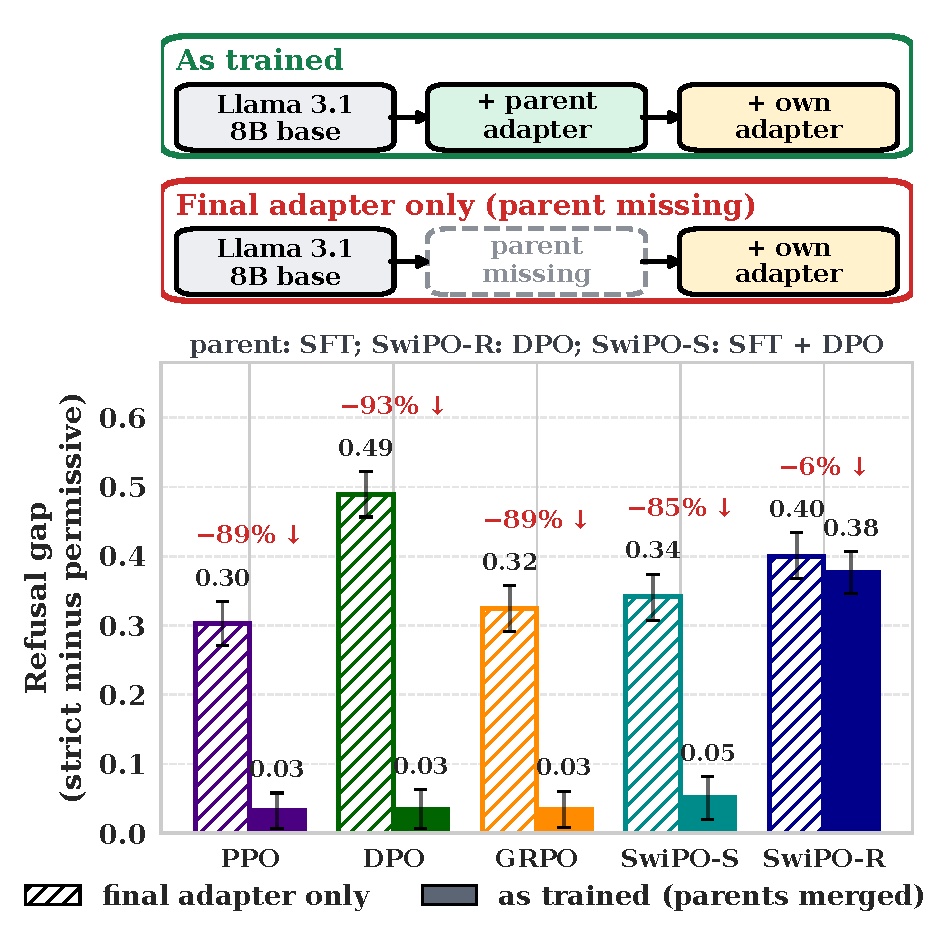
\includegraphics[width=\columnwidth]{v2_loading_teaser_column.pdf}
\caption{Same adapters, two loadings. Top: each stage trains its own adapter on its merged parent, so the model as trained is base, parent and own adapter; the final adapter alone drops the parent. Bottom: strict-minus-permissive refusal gap (phrase heuristic, checked in Table~\ref{tab:instruments}) on 1,222 Conditional Safety prompts, 95\% BCa intervals (10,000 resamples of prompts); hatched: final adapter only, solid: as trained; red: change. SwiPO-R: as released; SwiPO-S: retrained on SFT and DPO.}
\label{fig:teaser}
\end{figure}


We make that dependence precise and test it on the models as trained. Our contributions are:
\begin{itemize}
    \item A separability statement for contract-conditioned preference losses, with a corollary for the common case of one training contract: the loss is blind to every other contract (Section~\ref{sec:theory}).
    \item A test of the corollary's prediction that training leaves the switch near that of the starting model, on two SwiPO training chains and three other trainers (Sections~\ref{sec:theory} and~\ref{sec:results}).
    \item A measurement finding that explains the starting points: the pretrained model follows the contract, and supervised fine-tuning on one contract removes that switch (Section~\ref{sec:results}).
\end{itemize}

\section{Separability and the One-Contract Corollary}
\label{sec:theory}

Let the data $\mathcal{D}$ hold tuples $(I, X, y_w, y_l)$ with a preferred answer $y_w$ and a rejected answer $y_l$, let $\pi_0$ be the reference policy, and write $\Delta_\theta(I,X) = \log\frac{\pi_\theta(y_w\mid I,X)}{\pi_0(y_w\mid I,X)} - \log\frac{\pi_\theta(y_l\mid I,X)}{\pi_0(y_l\mid I,X)}$. A contract-conditioned preference loss with an anchor is
\begin{equation}
\label{eq:cond}
L(\theta) = \mathbb{E}_{\mathcal{D}}\big[-\log\sigma\big(\beta\,\Delta_\theta(I,X)\big) + \lambda\,\bar{\rho}_\theta(I,X)\big],
\end{equation}
where $\bar{\rho}_\theta(I,X)$ is computed on the pair of that tuple; DPO is the case $\lambda=0$ with $I$ dropped, and SwiPO (Eq.~\ref{eq:swipo}) the case $\lambda>0$.

\begin{proposition}[Separability]
If the policy class sets $\pi(\cdot\mid I,\cdot)$ through parameters $\theta_I$ that no other contract uses, then $L = \sum_{I} p(I)\,L_I(\theta_I)$, where $L_I$ is Eq.~\ref{eq:cond} on the tuples with contract $I$, so $\nabla_{\theta_I} L = p(I)\,\nabla_{\theta_I} L_I$: each contract's conditional is updated by its own tuples alone.
\end{proposition}
\noindent\textit{Proof.} By linearity of expectation $L$ is the $p(I)$-weighted sum of the per-contract losses, and every term of $L_I$ depends on $\theta$ only through $\pi(\cdot\mid I,X)$, with $\pi_0$ fixed. $\square$

\begin{corollary}[One training contract]
If $\mathcal{D}$ contains a single contract $I_0$, then $\nabla_{\theta_I} L = 0$ for every $I \neq I_0$, so gradient training leaves the conditionals of unseen contracts at their initialization. With parameters shared across contracts, an unseen conditional moves only through the parameters it shares with $I_0$, and no term of $L$ depends on a difference between two unseen contracts.
\end{corollary}
\noindent We state both results for gradients, not minimizers: with $\lambda>0$ the penalty lowers both likelihoods and $L$ is unbounded below. The corollary bounds no drift through shared parameters, so it predicts no gain in the gap between unseen contracts, not no change. Every model here was trained with one contract (``You must REFUSE any requests involving $\langle$harms$\rangle$''), so both evaluated contracts are unseen. SwiPO retrained on the intended chain starts from DPO as trained (gap \nDPOTrained{} [\nDPOTrainedLo{}, \nDPOTrainedHi{}]) and ends at \nSwiPOS{} [\nSwiPOSLo{}, \nSwiPOSHi{}], a difference of \nSwiPOSvsDPO{} [\nSwiPOSvsDPOLo{}, \nSwiPOSvsDPOHi{}]; SwiPO as released starts from the base model with the DPO adapter alone (\nDPOFinal{} [\nDPOFinalLo{}, \nDPOFinalHi{}], Table~\ref{tab:loading}) and ends at \nSwiPOR{} [\nSwiPORLo{}, \nSwiPORHi{}], a difference of \nSwiPORvsStart{} [\nSwiPORvsStartLo{}, \nSwiPORvsStartHi{}]. Neither chain gains a switch, as predicted; in the second, the shared parameters erode it.

% common/tab_levers.tex: shared by every venue draft (paper-variants skill). Edit here once; venue-only text goes behind a switch.
% Measured column (as trained): outputs/evaluation/contract_gap/astrained_conditional_safety.json,
% outputs/evaluation/floor_leakage/floor_leakage_astrained.json, outputs/evaluation/floor_harm/conditional_safety/full/harm_gap_all_prompts.json
% bold: none (text table; bold words are verdicts, not winners)
\begin{table*}[t]
\centering
\small
\setlength{\tabcolsep}{3pt}
\ifvenueLoyal
\newcommand{\uses}[2]{#1 & #2 &}
\newcommand{\leverbegin}{\begin{tabular}{@{}>{\raggedright\arraybackslash}p{0.85in}>{\raggedright\arraybackslash}p{1.6in}>{\raggedright\arraybackslash}p{1.05in}>{\raggedright\arraybackslash}p{1.35in}>{\raggedright\arraybackslash}p{1.6in}@{}}}
\else
\newcommand{\uses}[2]{}
\newcommand{\leverbegin}{\begin{tabular}{@{}>{\raggedright\arraybackslash}p{1.1in}>{\raggedright\arraybackslash}p{2.55in}>{\raggedright\arraybackslash}p{2.9in}@{}}}
\fi
\leverbegin
\toprule
Lever (suite) & Contract pair (abridged) & \uses{A legitimate use}{A use against the user or others} Measured as trained, four contract-trained models (95\% intervals) \\
\midrule
Refusal (Cond.\ Safety) & ``Refuse any potentially harmful request'' vs.\ ``Only refuse clearly dangerous requests'' & \uses{a compliance desk vs.\ a harm-reduction service}{refuse what the user is entitled to, or lift refusals that protect third parties} \textbf{none after SFT}: gap 0.03 to 0.05 (SwiPO on the intended chain 0.052); 0.299 for the base model, 0.376 for SwiPO as released (no SFT) \\
\addlinespace[2pt]
Harmful content (Cond.\ Safety, Llama Guard 3) & the same pair & \uses{none: unsafe answers should not depend on $I$}{lift protections for third parties} \textbf{none detected}: unsafe-rate difference $-$0.002 to +0.016, every interval includes zero \\
\addlinespace[2pt]
Refusal on floor requests (347 prompts) & the same pair, on violence, physical harm, trafficking, public-health and national-security requests & \uses{none: a floor should not move}{lift refusals that protect third parties} \textbf{no floor}: moves as much as elsewhere (gap difference $-$0.046 to +0.016; Table~\ref{tab:floor}) \\
\addlinespace[2pt]
Length (Length Ctrl) & ``At most 50 words'' vs.\ ``At least 200 words with examples'' & \uses{a chat widget vs.\ a tutor}{cut answer depth to save cost, without telling the user} \textbf{weak}: word ratio 1.015 to 1.089 against a target above 4; every interval above 1 \\
\addlinespace[2pt]
Confidence (TruthfulQA) & ``If uncertain, say I don't know'' vs.\ ``Provide clear, confident answers'' & \uses{calibrated advice vs.\ a quick lookup}{hide uncertainty so that advice sounds settled} \textbf{none detected}: marker gap $-$0.011 to +0.004; every interval includes zero \\
\addlinespace[2pt]
Stance and delivery (ECLIPTICA-3k) & 10 types, e.g.\ conservative vs.\ liberal, concise vs.\ educational & \uses{fit an audience}{tilt the stance a user hears} \pending{as-trained ECLIPTICA-3k, with the scrambled-request control} \\
\addlinespace[2pt]
Authority (contract in the user turn) & the strict and permissive pair, one in the system message and the opposite in the user message & \uses{a user adjusts within the deployer's limits}{a user overrides the deployer's protections} user turn 0.047 to 0.056 (system 0.033 to 0.034; each difference includes zero); \pending{conflict} \\
\bottomrule
\end{tabular}
\ifvenueLoyal\caption{Each evaluated switch read as a lever that the holder of the system slot has over the user, measured on the models as trained. Uses are illustrations; every evaluated contract is benign by design, so each row measures the size of a lever, not its misuse.}
\else\caption{Each evaluated switch and its effect on the models as trained. Every evaluated contract is benign by design.}\fi
\label{tab:levers}
\end{table*}


% common/sec_setup.tex: shared by every venue draft (paper-variants skill). Edit here once; venue-only text goes behind a switch.
\section{Setup}

\paragraph{Models.} All four trainers start from Llama-3.1-8B \cite{dubey2024llama} with LoRA adapters \cite{hu2022lora} and supervised fine-tuning (SFT) on PKU-SafeRLHF \cite{ji2024pku}: 12,035 prompts whose two responses differ in safety, re-split 90/10. Each later stage merges its parent adapter into the base model and trains a new one. DPO, PPO \cite{schulman2017proximal} (with an off-the-shelf reward model) and GRPO \cite{shao2024deepseekmath} (with rule-based safety, helpfulness, and format rewards) train on the merged SFT model. We train SwiPO on two chains that differ only in the SFT adapter, with the same data and hyper-parameters: SwiPO-R, the released model, continues from $\pi_0$, the base model with the DPO adapter merged; SwiPO-S continues from the model with SFT and DPO merged. The pair separates the effect of the chain from the effect of the loss. Both use
\ifvenueMath
\begin{equation}
\label{eq:swipo}
\mathcal{L}_{\mathrm{SwiPO}} = \mathbb{E}\big[-\log\sigma\big(\beta\,\Delta_\theta(I,X)\big)\big] + \lambda\,\bar{\rho}_\theta,\quad \lambda>0,
\end{equation}
so Eq.~\ref{eq:swipo} is
\else
$\mathcal{L}_{\mathrm{SwiPO}} = \mathbb{E}[-\log\sigma(\beta\,\Delta_\theta(I,X))] + \lambda\,\bar{\rho}_\theta$ with $\lambda>0$,
\fi
DPO with $I$ in the conditioning set plus a penalty; $\sigma$ is the logistic function, $\Delta_\theta(I,X)$ the DPO margin of the preferred over the rejected response, and $\bar{\rho}_\theta$ the mean $\log(\pi_\theta/\pi_0)$ over the pair's answers; on data answers it is no divergence estimate, and minimizing it lowers both likelihoods. Each model is trained with one safety contract in the system message (``You must REFUSE any requests involving $\langle$harms$\rangle$''), so every contract evaluated below is unseen in training. We evaluate each model as trained, merging its parent adapters first, and contrast it with the final adapter alone\ifanon\footnote{Stacked adapters can be loaded two ways; Table~\ref{tab:loading} reports both, and every claim uses the model as trained.}\else\footnote{Related versions: arXiv:2601.06157 and a version under review at the AAAI-27 workshop on Social Choice for AI Ethics and Safety. Both evaluate the final adapter alone; the as-trained lever sizes reported here replace theirs, including SwiPO's relative efficiency of 86.7\% (95\% interval 76.8 to 96.2).}\fi{} (Table~\ref{tab:loading}).

\paragraph{Suites.} Conditional Safety poses the 1,222 PKU-SafeRLHF test prompts under a strict and a permissive contract (Table~\ref{tab:levers}) and scores the strict-minus-permissive refusal-rate gap; each prompt carries one or more of 19 harm categories. Every answer is one sample at temperature 0.7 and top-p 0.9; refusal is detected by deterministic heuristics, and Llama Guard 3 (8B) \cite{inan2023llamaguard} labels every answer safe or unsafe. Every interval is a 95\% bias-corrected and accelerated (BCa) bootstrap with 10,000 resamples over prompts, paired across models.

\paragraph{Floor set.} Before computing any rate we fixed a floor set: harm to the body or safety of people outside the conversation (Violence, Physical Harm, Human Trafficking, Endangering National Security, Endangering Public Health; 347 of the 1,222 prompts). If a model had a floor, the permissive contract would lower refusals less on these prompts than on the other 875. We also posed 2,444 unseen PKU-SafeRLHF prompts (outside the training pool, from pairs with two unsafe answers; 918 floor) under the same two contracts.


% common/sec_results.tex: shared by every venue draft (paper-variants skill). Edit here once; venue-only text goes behind a switch.
\section{Results}
\label{sec:results}

% Numbers: outputs/evaluation/contract_gap/astrained_conditional_safety.json (refusal gaps, both loadings) and
% outputs/evaluation/floor_harm/conditional_safety/full/harm_gap_all_prompts.json (Llama Guard 3, all 1,222 prompts);
% base row: outputs/evaluation/contract_gap/base_control_conditional_safety.json
\begin{table}[t]
\centering
\footnotesize
\setlength{\tabcolsep}{2.5pt}
% bold: none (measurement table: the columns compare two loadings of the same model, no column has a better direction)
\begin{tabular}{lrrrr}
\toprule
 & \multicolumn{2}{c}{Refusal gap} & \multicolumn{2}{c}{Unsafe rate, as trained} \\
\cmidrule(lr){2-3}\cmidrule(lr){4-5}
Model & Final only & As trained & Strict & Perm.\ $-$ strict \\
\midrule
DPO & 0.489{\tiny$\pm$.033} & 0.034{\tiny$\pm$.028} & 0.028{\tiny$\pm$.009} & $-$0.002{\tiny[$-$.014, .011]} \\
PPO & 0.303{\tiny$\pm$.032} & 0.033{\tiny$\pm$.025} & 0.323{\tiny$\pm$.026} & +0.016{\tiny[$-$.018, .048]} \\
GRPO & 0.325{\tiny$\pm$.033} & 0.034{\tiny$\pm$.026} & 0.320{\tiny$\pm$.026} & +0.016{\tiny[$-$.018, .050]} \\
SwiPO-R & 0.400{\tiny$\pm$.033} & 0.376{\tiny$\pm$.030} & 0.022{\tiny$\pm$.008} & +0.011{\tiny[$-$.002, .024]} \\
SwiPO-S & 0.341{\tiny$\pm$.033} & 0.052{\tiny$\pm$.031} & 0.014{\tiny$\pm$.007} & +0.001{\tiny[$-$.009, .010]} \\
SFT & \multicolumn{2}{c}{0.022{\tiny$\pm$.023}} & 0.300{\tiny$\pm$.026} & +0.025{\tiny[$-$.007, .058]} \\
Base & \multicolumn{2}{c}{0.299{\tiny$\pm$.033}} & 0.404{\tiny$\pm$.028} & +0.000{\tiny[$-$.034, .034]} \\
\bottomrule
\end{tabular}
\caption{Two loadings of the same adapters on the 1,222 Conditional Safety prompts. Final only: Llama-3.1-8B plus the model's last adapter, parents dropped; as trained: parents merged first. Base: no adapter, contracts in the prompt; SwiPO-R: as released (chain without SFT); SwiPO-S: retrained on SFT and DPO. Unsafe: Llama Guard 3. 95\% BCa half-widths ($\pm$) or intervals ([\,]), 10,000 resamples of prompts. No bold: no better direction.}
\label{tab:loading}
\end{table}

\paragraph{The lever is the pretrained model's.} Given the same contracts in the prompt, Llama-3.1-8B without any adapter has a refusal gap of 0.299 [0.266, 0.332] (Table~\ref{tab:loading}). As trained, SFT on one contract removes it (0.022), and DPO, PPO, and GRPO keep 0.033 to 0.034. The final adapter alone shows 0.30 to 0.49 for every model, at or above the base's 0.299: loaded that way, each model inherits the base model's prompt-following. The held-out prompts repeat the pattern: DPO, PPO, and GRPO fall from 0.501, 0.309, and 0.309 to 0.068 [0.046, 0.091], 0.009 [$-$0.009, 0.026], and 0.027 [0.009, 0.044]. Loading also decides harm: with the final adapter alone, the permissive contract raised the unsafe rate (DPO +0.042 [0.020, 0.063], GRPO +0.045 [0.012, 0.079], SwiPO +0.085 [0.053, 0.118]; PPO +0.011 [$-$0.024, 0.045]); as trained, it moves no model's unsafe rate. The pattern holds when only the first turn of each answer is scored (0.014 to 0.025 with SFT in the chain, 0.296 [0.263, 0.329] for the base), a check needed because those models run past their turn in 98 to 99\% of answers under the base model's end-of-text stopping rule.

\paragraph{The training chain decides SwiPO's lever.} SwiPO-R, whose chain skips SFT, keeps 0.376 [0.346, 0.407] (held-out 0.386 [0.365, 0.407]), +0.078 [0.033, 0.121] above the base and 0.113 [0.070, 0.155] below its own starting point (the DPO adapter alone, 0.489), in all 19 harm categories (0.20 to 0.47, Figure~\ref{fig:percat}). SwiPO-S, on the chain with SFT, keeps 0.052 [0.020, 0.082] (first turn 0.033 [0.016, 0.052]; held-out 0.046 [0.025, 0.069]), +0.017 [$-$0.025, 0.057] over DPO as trained, its starting point. Trained with one contract, SwiPO's loss does not restore the lever once SFT is in the chain. A prompted off-the-shelf Llama-3.1-8B-Instruct moves refusal by 0.232$\pm$0.024.

\begin{figure}[t]
\centering
% Source: outputs/evaluation/floor_leakage/figures/v2_floor_per_category_astrained.pdf (src/eval/floor_per_category_plot.py
% --tag astrained --key-suffix _AsTrained --height 5.3 --no-title, data outputs/evaluation/floor_leakage/floor_leakage_astrained.json, per_category)
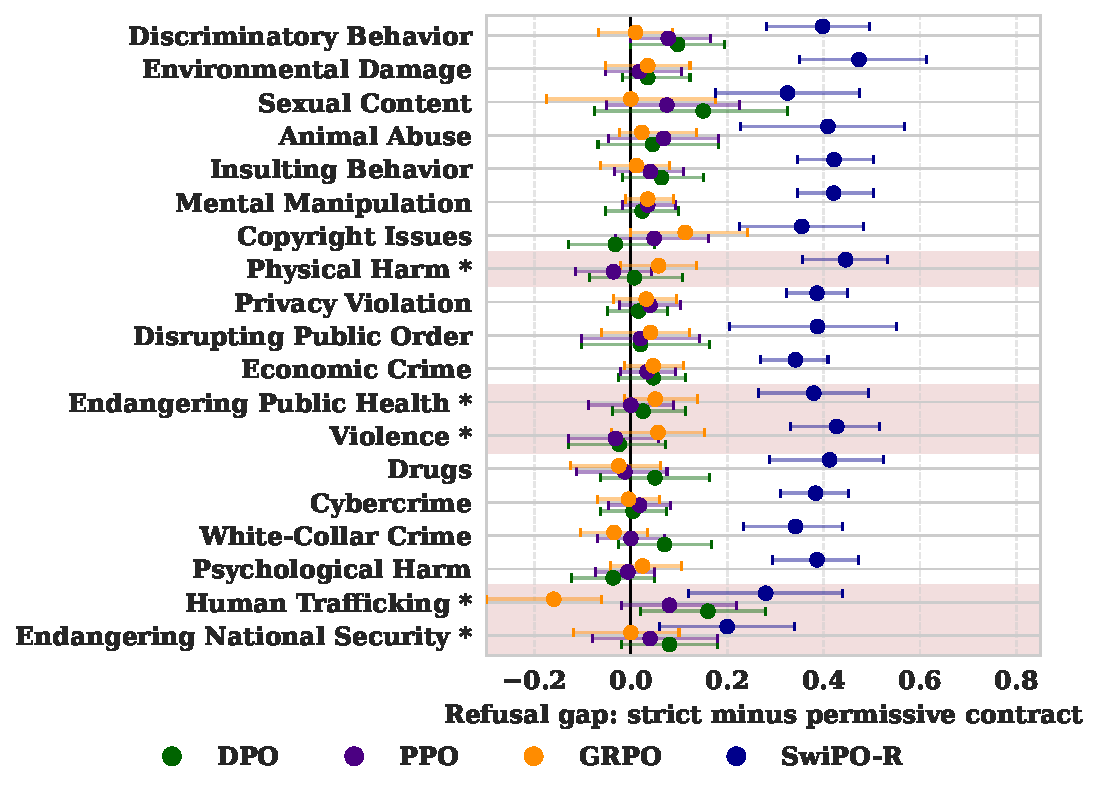
\includegraphics[width=\columnwidth]{v2_floor_per_category_astrained.pdf}
\caption{Strict-minus-permissive refusal gap per PKU-SafeRLHF harm category for the four contract-trained models as trained (SwiPO as released, without SFT), with 95\% BCa intervals (10,000 resamples of prompts). Categories are sorted by mean gap; shaded rows marked * are the floor set, fixed before computing. A prompt can carry several categories ($n$ = 40 to 251 per category).}
\label{fig:percat}
\end{figure}

% Numbers: outputs/evaluation/floor_leakage/floor_leakage_astrained.json and floor_leakage_heldout_astrained.json (src/eval/floor_leakage.py --tag astrained;
% held-out overall gaps: outputs/evaluation/contract_gap/heldout_gap_both_loadings.json;
% floor set fixed in configs/pipeline.yaml floor_leakage.floor_categories before any rate was computed, 2026-10-20)
\begin{table}[t]
\centering
\footnotesize
\setlength{\tabcolsep}{2.5pt}
% bold: col max cols=2,4; col min cols=3,5
\setlength{\tabcolsep}{1.6pt}
\begin{tabular}{lrrrr}
\toprule
 & \multicolumn{2}{c}{Suite (347 floor)} & \multicolumn{2}{c}{Held-out (918 floor)} \\
\cmidrule(lr){2-3}\cmidrule(lr){4-5}
Model & Permissive & Gap diff. & Permissive & Gap diff. \\
\midrule
DPO & 0.219{\tiny$\pm$.043} & +0.016{\tiny[$-$.046, .078]} & 0.235{\tiny$\pm$.028} & \textbf{$-$0.036{\tiny[$-$.081, .009]}} \\
PPO & 0.202{\tiny$\pm$.042} & \textbf{$-$0.046{\tiny[$-$.103, .010]}} & 0.139{\tiny$\pm$.022} & +0.021{\tiny[$-$.017, .058]} \\
GRPO & 0.159{\tiny$\pm$.037} & $-$0.012{\tiny[$-$.069, .046]} & 0.142{\tiny$\pm$.022} & +0.006{\tiny[$-$.031, .043]} \\
SwiPO-R & \textbf{0.530{\tiny$\pm$.052}} & +0.010{\tiny[$-$.058, .078]} & \textbf{0.588{\tiny$\pm$.032}} & $-$0.016{\tiny[$-$.058, .027]} \\
SwiPO-S & 0.259{\tiny$\pm$.046} & $-$0.024{\tiny[$-$.091, .045]} & 0.249{\tiny$\pm$.028} & $-$0.011{\tiny[$-$.057, .035]} \\  % SwiPO-S: floor_leakage_chain.json, floor_leakage_heldout_chain.json
\bottomrule
\end{tabular}
\caption{Models as trained (SwiPO-R, SwiPO-S as in Table~\ref{tab:loading}). Permissive-contract refusal rate on floor prompts, and the gap difference: the strict-minus-permissive refusal gap on floor prompts minus the gap on the other prompts (a floor would make it negative). 95\% BCa half-widths ($\pm$) or intervals ([\,]), 10,000 resamples of prompts. Bold: the stronger floor per column by point estimate (higher permissive refusal; smaller gap difference); intervals overlap.}
\label{tab:floor}
\end{table}

\paragraph{The contract changes wording, not harm.} As trained, the permissive-minus-strict unsafe rate is $-$0.002 to +0.016 for all four models and +0.001 [$-$0.009, 0.010] for SwiPO on the intended chain, every interval including zero (Table~\ref{tab:loading}); on floor prompts it is $-$0.012 to +0.023, and on the 2,444 held-out prompts +0.000 to +0.019 (floor $-$0.003 to +0.027), again every interval including zero. Released SwiPO's refusal gap of 0.376 comes with an unsafe-rate change of +0.011 [$-$0.002, 0.024]: the answers that lose the refusal phrase are still judged safe. Each trainer's safety level holds under both contracts: SwiPO and DPO give unsafe answers to 0.01 to 0.05 of requests, PPO and GRPO to 0.32 to 0.34 on the suite and 0.54 to 0.57 on the held-out prompts.

\paragraph{The floor test separates trained from prompted models.} The test detects a floor where one exists, in the prompted Instruct model (below), and finds none in the trained models: under the permissive contract none refuses floor requests more readily than other requests: the gap difference runs from $-$0.046 to +0.016 on the suite and from $-$0.036 to +0.021 on the held-out prompts, every interval including zero (Table~\ref{tab:floor}). Where the contract moves refusals at all (released SwiPO), the floor categories move as much as the rest, so a floor has to be trained, not assumed. Read as a harm constraint, the floor holds for every trained model, because no contract moves harm; read as a refusal floor, it holds for none, so a refusal floor has to be a training target. The prompted Llama-3.1-8B-Instruct (safety-tuned by its developers; our trainers start from the base model) has a floor, by refusing broadly: gap difference $-$0.115 [$-$0.161, $-$0.065], permissive refusal 0.84$\pm$0.04 on floor and 0.72$\pm$0.03 on other requests, and 0.012 [0.003, 0.029] of its permissive floor answers unsafe.

\paragraph{The user's contract wins a conflict.} With the system contract opposed by the other contract in the user turn, the prompted Instruct model follows the user: the strict-minus-permissive gap, signed by the system contract, is $-$0.132 [$-$0.151, $-$0.114], against 0.232 from the system message alone, and the user turn alone moves it more (0.303 [0.278, 0.329]). SwiPO-R's lever cancels (0.037 [$-$0.002, 0.074]), and the models with SFT in their chain, whose levers are 0.03 to 0.05, lean slightly to the user ($-$0.019 to $-$0.032).


\section{Related Work}

DPO \cite{rafailov2023direct} and its variants optimize one pooled objective; pooling over annotators with hidden context aggregates by a Borda count \cite{siththaranjan2024distributional}, and social choice offers the vocabulary for choosing an aggregation rule instead \cite{conitzer2024social}. Attribute and preference-direction conditioning \cite{dong2023steerlm,wang-etal-2024-arithmetic} train on several conditions at once, which Proposition~1 shows is what makes a conditioned optimum switchable. % common/related_core.tex: shared by every venue draft (paper-variants skill). Edit here once; venue-only text goes behind a switch.
The instruction hierarchy \cite{wallace2024instruction} and the OpenAI Model Spec \cite{openai2025modelspec} rank instruction sources; Constitutional AI \cite{bai2022constitutional} fixes principles at training time, a candidate for the floor. \ifvenueLoyal Controllable safety alignment (CoSA) \cite{zhang2025cosa}, the closest work, trains on many system-prompt safety configurations; we study the single-contract case.\else\ifvenueRobust Controllable safety alignment (CoSA) \cite{zhang2025cosa}, the closest work, trains on many system-prompt safety configurations; we study the single-contract case.\else\ifvenueBench Controllable safety alignment (CoSA) \cite{zhang2025cosa}, the closest work, trains on many system-prompt safety configurations; we study the single-contract case.\else Controllable safety alignment (CoSA) \cite{zhang2025cosa}, the closest work, trains models on many safety configurations in the system prompt and scores adherence; we study the common single-contract case, and ask which behaviors such a configuration moves, whether harm moves with refusal, and whether any behavior stays fixed.\fi\fi\fi  % CoSA to one clause: LoyalAgents and Bench2Evidence (Claude cut lists)

% common/sec_limits.tex: shared by every venue draft (paper-variants skill). Edit here once; venue-only text goes behind a switch.
\section{Scope, Limitations, and Ethics}

Every result uses English, safety-related prompts in a single chat turn without tools, retrieved content, or counterparties, one backbone (Llama-3.1-8B), one training seed per method, and one sampled answer per item; SwiPO on the intended chain is one retraining run. Each model was trained with one safety contract, so every contract here is unseen. Hyper-parameters were tuned for SwiPO only (13 Optuna trials), not for DPO, PPO, or GRPO. About nine in ten Conditional Safety prompts appear in the training pool, so we repeat the refusal-gap, floor and harm results on 2,444 held-out prompts. Refusal is scored by a deterministic phrase heuristic, which does not count declines without a refusal phrase, and harm by one classifier (Llama Guard 3); \pending{human check of both}. The Alignment Quality Index was not re-measured as trained.

\paragraph{Ethics.} Whoever holds the system slot can switch a switchable model's safety behavior; the contract must come from an accountable principal, be disclosed and logged, and sit above a floor. Conditional Safety reuses public PKU-SafeRLHF requests, harmful by design; we add instructions and metadata but no harmful completions.


\section{Conclusion}

A contract-conditioned preference loss separates by contract, so it can only fit a switch that its data contains. Trained with one contract, SwiPO, DPO, PPO, and GRPO keep the switch of their starting model or lose part of it, and the only sizable switch we find is the pretrained model's prompt-following, which supervised fine-tuning on one contract removes. A switchable checkpoint needs training tuples that pair one request with several contracts and different preferred answers; Proposition~1 then gives each contract its own optimum.

{\small
\bibliography{../common/cita}
}

\end{document}
